\documentclass[11pt]{standalone}
\usepackage{amssymb}
\usepackage{amsmath}
\usepackage[no-math]{fontspec}
\usepackage{unicode-math}
\setmainfont{Libertinus Sans}
\setsansfont{Libertinus Sans}
\setmathfont{Libertinus Math}
\usepackage{pgf,xcolor}
\usepackage{tikz}
\usetikzlibrary{arrows.meta, backgrounds, calc}
\usepackage{pgfplots}
\pgfplotsset{compat=newest}
\usepackage{pifont}

\definecolor{my_darkgray}{HTML}{484949}
\definecolor{my_lightgray}{HTML}{F3F4F4}
\definecolor{my_darkblue}{HTML}{005A94}
\definecolor{my_lightblue}{HTML}{CCDEE9}
\definecolor{my_yellow}{HTML}{FFEC7F}
\definecolor{my_red}{HTML}{E60000}
\definecolor{my_orange}{HTML}{E87846}

\begin{document}
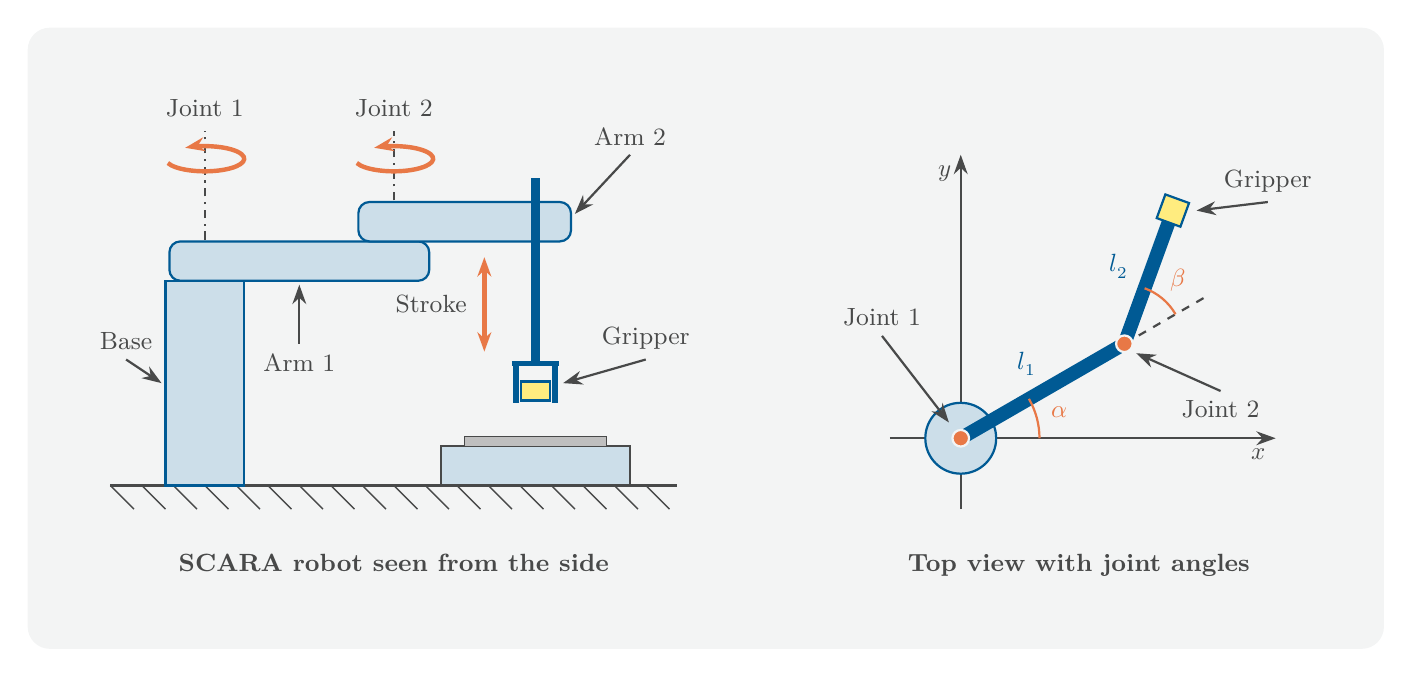
\begin{tikzpicture}[
    show background rectangle,
    background rectangle/.style={fill=my_lightgray, rounded corners=8pt},
    inner frame sep=0.8cm,
    annotation/.style={draw=my_darkgray, thick, -{Stealth[length=7pt, width=5pt]}},
    drehpfeil/.style={draw=my_orange, ultra thick, -{Stealth[length=7pt, width=5pt]}}
]

    % Maßstab: 1 m = 6 cm, also l_1 = 0.4 m = 2.4 cm und l_2 = 0.3 m = 1.8 cm

    % ===== Panel 1: SCARA-Roboter von der Seite =====
    \begin{scope}

        % Boden mit Schraffur
        \draw[draw=my_darkgray, thick] (-1.2,0) -- (6.0,0);
        \foreach \x in {-1.2,-0.8,...,5.6} {
            \draw[draw=my_darkgray, line width=0.5pt] (\x,0) -- ++(0.3,-0.3);
        }

        % Werkstückträger mit Platine unter dem Greifer
        \draw[fill=my_lightblue, draw=my_darkgray, thick] (3.0,0) rectangle (5.4,0.5);
        \draw[fill=my_darkgray!35, draw=my_darkgray] (3.3,0.5) rectangle (5.1,0.62);

        % Drehachsen der beiden Gelenke (strichpunktiert)
        \draw[draw=my_darkgray, thick, dash dot] (0,2.3) -- (0,4.5);
        \draw[draw=my_darkgray, thick, dash dot] (2.4,2.8) -- (2.4,4.5);

        % Sockel
        \draw[fill=my_lightblue, draw=my_darkblue, thick] (-0.5,0) rectangle (0.5,2.6);

        % Arm 1 (Gelenk 1 bis Gelenk 2) und Arm 2 (Gelenk 2 bis Greifer)
        \draw[fill=my_lightblue, draw=my_darkblue, thick, rounded corners=4pt]
            (-0.45,2.6) rectangle (2.85,3.1);
        \draw[fill=my_lightblue, draw=my_darkblue, thick, rounded corners=4pt]
            (1.95,3.1) rectangle (4.65,3.6);

        % Hubachse mit Greifer und Bauteil
        \draw[draw=my_darkblue, line width=3pt] (4.2,3.9) -- (4.2,1.55);
        \draw[draw=my_darkblue, line width=2pt] (3.9,1.55) -- (4.5,1.55);
        \draw[draw=my_darkblue, line width=2pt] (3.95,1.55) -- (3.95,1.05);
        \draw[draw=my_darkblue, line width=2pt] (4.45,1.55) -- (4.45,1.05);
        \draw[fill=my_yellow, draw=my_darkblue, thick] (4.02,1.08) rectangle (4.38,1.32);

        % Drehbewegung der Gelenke um die senkrechten Achsen
        \draw[drehpfeil] ($(0,4.15)+(200:0.5 and 0.16)$)
            arc[start angle=200, end angle=480, x radius=0.5, y radius=0.16];
        \draw[drehpfeil] ($(2.4,4.15)+(200:0.5 and 0.16)$)
            arc[start angle=200, end angle=480, x radius=0.5, y radius=0.16];
        \node[font=\small, text=my_darkgray, anchor=south] at (0,4.55) {Joint 1};
        \node[font=\small, text=my_darkgray, anchor=south] at (2.4,4.55) {Joint 2};

        % Hubbewegung der senkrechten Achse
        \draw[draw=my_orange, ultra thick,
              {Stealth[length=7pt, width=5pt]}-{Stealth[length=7pt, width=5pt]}]
            (3.55,1.7) -- (3.55,2.9);
        \node[font=\small, text=my_darkgray, anchor=east] at (3.45,2.3) {Stroke};

        % Beschriftungen
        \draw[annotation] (-1.0,1.6) -- (-0.55,1.3);
        \node[font=\small, text=my_darkgray, anchor=south] at (-1.0,1.6) {Base};
        \draw[annotation] (1.2,1.8) -- (1.2,2.55);
        \node[font=\small, text=my_darkgray, anchor=north] at (1.2,1.8) {Arm 1};
        \draw[annotation] (5.4,4.2) -- (4.7,3.45);
        \node[font=\small, text=my_darkgray, anchor=south] at (5.4,4.2) {Arm 2};
        \draw[annotation] (5.6,1.6) -- (4.55,1.3);
        \node[font=\small, text=my_darkgray, anchor=south] at (5.6,1.6) {Gripper};

        \node[font=\small\bfseries, text=my_darkgray, anchor=north]
            at (2.4,-0.75) {SCARA robot seen from the side};
    \end{scope}

    % ===== Panel 2: Draufsicht mit Gelenkwinkeln =====
    \begin{scope}[xshift=9.6cm, yshift=0.6cm]

        % Gelenk 1 im Ursprung, alpha = 30 Grad, beta = 40 Grad
        \coordinate (G1) at (0,0);
        \coordinate (G2) at (30:2.4);
        \coordinate (GR) at ($(G2)+(70:1.8)$);

        % Koordinatenachsen
        \draw[draw=my_darkgray, thick, -{Stealth[length=7pt, width=5pt]}] (-0.9,0) -- (4.0,0)
            node[anchor=north east, font=\small, text=my_darkgray] {$x$};
        \draw[draw=my_darkgray, thick, -{Stealth[length=7pt, width=5pt]}] (0,-0.9) -- (0,3.6)
            node[anchor=north east, font=\small, text=my_darkgray] {$y$};

        % Sockel von oben
        \draw[fill=my_lightblue, draw=my_darkblue, thick] (G1) circle (0.45);

        % Verlängerung von Arm 1 als Bezug für beta
        \draw[draw=my_darkgray, thick, dashed] (G2) -- ($(G2)+(30:1.2)$);

        % Arme
        \draw[draw=my_darkblue, line width=5pt, line cap=round] (G1) -- (G2) -- (GR);

        % Winkel alpha und beta
        \draw[draw=my_orange, thick] (1.0,0) arc[start angle=0, end angle=30, radius=1.0];
        \node[font=\small, text=my_orange] at (15:1.3) {$\alpha$};
        \draw[draw=my_orange, thick] ($(G2)+(30:0.75)$) arc[start angle=30, end angle=70, radius=0.75];
        \node[font=\small, text=my_orange] at ($(G2)+(50:1.05)$) {$\beta$};

        % Armlängen
        \node[font=\small, text=my_darkblue] at ($(G1)!0.5!(G2)+(120:0.4)$) {$l_1$};
        \node[font=\small, text=my_darkblue] at ($(G2)!0.5!(GR)+(160:0.4)$) {$l_2$};

        % Gelenke und Greifer mit Bauteil
        \foreach \P in {G1, G2} {
            \draw[fill=my_orange, draw=my_lightgray, thick] (\P) circle (3pt);
        }
        \node[draw=my_darkblue, fill=my_yellow, thick, minimum size=0.32cm,
              inner sep=0pt, rotate=70] at (GR) {};

        % Beschriftungen
        \draw[annotation] (-1.0,1.3) -- (-0.15,0.2);
        \node[font=\small, text=my_darkgray, anchor=south] at (-1.0,1.3) {Joint 1};
        \draw[annotation] (3.3,0.6) -- ($(G2)+(0.15,-0.12)$);
        \node[font=\small, text=my_darkgray, anchor=north] at (3.3,0.6) {Joint 2};
        \draw[annotation] (3.9,3.0) -- ($(GR)+(0.3,0)$);
        \node[font=\small, text=my_darkgray, anchor=south] at (3.9,3.0) {Gripper};

        \node[font=\small\bfseries, text=my_darkgray, anchor=north]
            at (1.5,-1.35) {Top view with joint angles};
    \end{scope}

\end{tikzpicture}
\end{document}
